\chapter{Глава 6}

В очередной раз рад приветствовать своих читателей. Новый эпизод японской серии подоспел. В прошлый раз мы остановились на японском участии в Версальской конференции. Как мы помним, маркиз Сайондзи Киммоти сумел отстоять позиции Японии по ключевому для неё вопросу о Шаньдуне и в целом Китае. Статья 156 Версальского договора гласила, что Германская империя отказывается от прав на Шаньдун не в пользу Китая, а в пользу Японии. Сохраняли силу и 16 пунктов, и вообще весь комплекс японо-китайских договорённостей. Судя по всему, во имя этого японцам пришлось согласиться на большую солидарность с общеантантовской линией в России – но о нашей стране мы ещё поговорим позже.

Пока же стоит взглянуть на Поднебесную и на то, как там отозвались перипетии Версаля. Сам Договор, как известно, был подписан 28 июня 1919. Но Китая среди подписантов не было – по существу имел место демонстративный бойкот, что не могло добавить очков Пекинскому правительству в глазах ведущих мировых держав. В сентябре 1919 года Китай просто объявил о прекращении состояния войны с Германией. Формальный же сепаратный мирный договор с Германией будет подписан только в 1921. Впрочем, куда важнее то, что произошло в связи со всем этим внутри Поднебесной. Мы помним о том, что единство страны носило иллюзорный, фиктивный характер – враждующие между собой клики были вынуждены изображать его, чтобы избежать пожирания страны по кускам (что легко могло случиться, объяви эти куски о независимости) разного рода империалистическими хищниками – в первую очередь, конечно, японцами, но не только ими. Единственным способом не оказаться съеденными, было оставаться чересчур большими, чтобы кто-бы то ни было мог проглотить и переварить без несварения и неприятных международных последствий со стороны конкурентов такой большой объём территории и населения. Но вот подсидеть друг друга, занять доминирующее положение, стать лицом страны, получая от этого все возможные плюшки, клики были готовы и даже очень. И доминировавшие (и то относительно) после смерти Юань Шикая Аньхойцы нипочём не стали бы злить сильных мира сего, приобретать репутацию недоговороспособных, а значит буквально заставлять внешних игроков сделать ставку на кого-то другого во внутрикитайской игре. Нет, конечно, руководители клики не возражали бы, если бы уловка с “тоже воевавшим” в ПМВ Китаем смогла принести плоды и покончить с японскими привилегиями и притязаниями. Лидер Аньхойцев Дуань Цижуй хотя и считался японским ставленником и сторонником (это даже привело к тому, что ввиду интриг и под влиянием других держав – в частности США, опасавшихся его чрезмерной прояпонскости, он был вынужден формально уйти в отставку с поста премьер-министра в конце 1918, хотя и сохранил определяющее влияние на дела), в действительности просто брал из той руки, которая были готова давать, и которая могла очень больно ударить, если попытаться куснуть её. Но, безусловно, ни он, ни другая, возвышающаяся в этот период политическая фигура – видный деятель Чжилийской клики и президент страны с августа 1917 по сентябрь 1918 Фэн Гочжан никогда не стали бы публично харкать в лицо собравшимся в Версале победителям, если бы у них оставался хоть какой то иной выбор. Его просто не было.

Итоги Версаля для страны (и, конечно, Великий Октябрь – про него тоже забывать не стоит) привели к тому, что Китай закипел. Впрочем, о так называемом “Движении 4 мая” стоит сказать несколько подробнее. Своё название оно получило по дате, когда впервые стало известно, что Шаньдунский вопрос Парижская мирная конференция собирается решить в пользу Японии, и антияпонская направленность сохранялась вплоть до конца его активного существования. Но в реальности цели и смысл Движения были гораздо шире. Синьхайская революция, помимо глубоких социально-экономических факторов, была вызвана тем, что Китай, продолжая на словах вплоть до конца правления императрицы Цыси кичиться своим древним величием, в действительности с середины XIX столетия шёл через почти непрерывную полосу поражений, причём, что особенно важно, поражений унизительных, указывающих на общую отсталость. Попытка традиционалистов и защитников старины восстать не только против врагов страны, но и против всего, что они несли, а фактически – против внешнего экономического проникновения и самого технического прогресса, отводившего старому Китаю роль периферии – выступление Ихэтуаней, окончилось полным крахом. Свержение Манчжурской династии и новое, республиканское устройство должны были вывести страну на путь всестороннего развития, а в реальности привели к её расколу. Но, что очень важно, этот раскол был не по какому-либо идеологическому принципу, не на основе глубоких социально-экономических различий. Клики были совершенно не похожи на красных и белых, или даже на северян и южан США (хотя в Китае тоже наблюдались некоторые различия – Юг в целом был несколько более развит и несколько более революционен), они группировались по принципу общности сослуживцев, землячеству, по факту уже почти клановому. Аньхоец или Чжилиец он скорее урождённый, чем убеждённый.

К началу 1919 года интеллектуалы Китая, а также та часть его экономических элит, которая не смогла присоединиться и получить гарантии безопасности ни от одной из крупных клик, не хотели больше жить по-старому. Отсутствие элементарной стабильности, милитаризация и внутренние войны, порождённые борьбой клик, вели к жесткому кризису и культуры, и экономики. И главное – ни одна из этих клик не смогла обеспечить уважение к Поднебесной и её нуждам на международной арене. Китайцы в Китае всегда и во всём, как и прежде, должны были тесниться перед иностранцами. Наиболее светлые головы хорошо понимали – с окончанием мировой войны, лишь только экономики реальных её участников перестроятся на мирный лад, Поднебесную затопят иностранные товары, окончательно уничтожив всякие шансы приподняться национальному производителю, а рассчитываться за них будут долгосрочными ресурсными концессиями. Причём к власти в Пекине будет приводиться та из клик, которая создаст лучшие условия для зарубежного капитала. Стране требовался новый и масштабный виток модернизации. Все здоровые силы сошлись на этом. В то же самое время и по тем же причинам войн клик и внутренней раздробленности продолжало ухудшаться и положения рабочих и крестьянских масс, которые уже просто не могли выносить сложившееся положение. В некоторые регионы в 1919 уже стали приходить, реализуя механизм 16 пунктов, японцы, что вызывало и закономерные, и преувеличенные опасения их жителей. Большое количество простых китайцев стало смотреть на ситуацию таким образом, что правящие группировки как минимум бессильны их защитить, а как максимум находятся в сговоре с Японией и другими заинтересованными странами.

В итоге сочетание недовольства низов и верхов, образованных и неграмотных рвануло с мощностью бомбы. До того, зачастую, те и другие действовали в рассинхроне. Теперь же… Началось всё 4 мая 1919 года в Пекине студенческой демонстрацией протеста против решений Парижской конференции и против предательства национальных интересов Китая продажными деятелями Пекинского правительства. 

\begin{figure}[h!tb] 
	\centering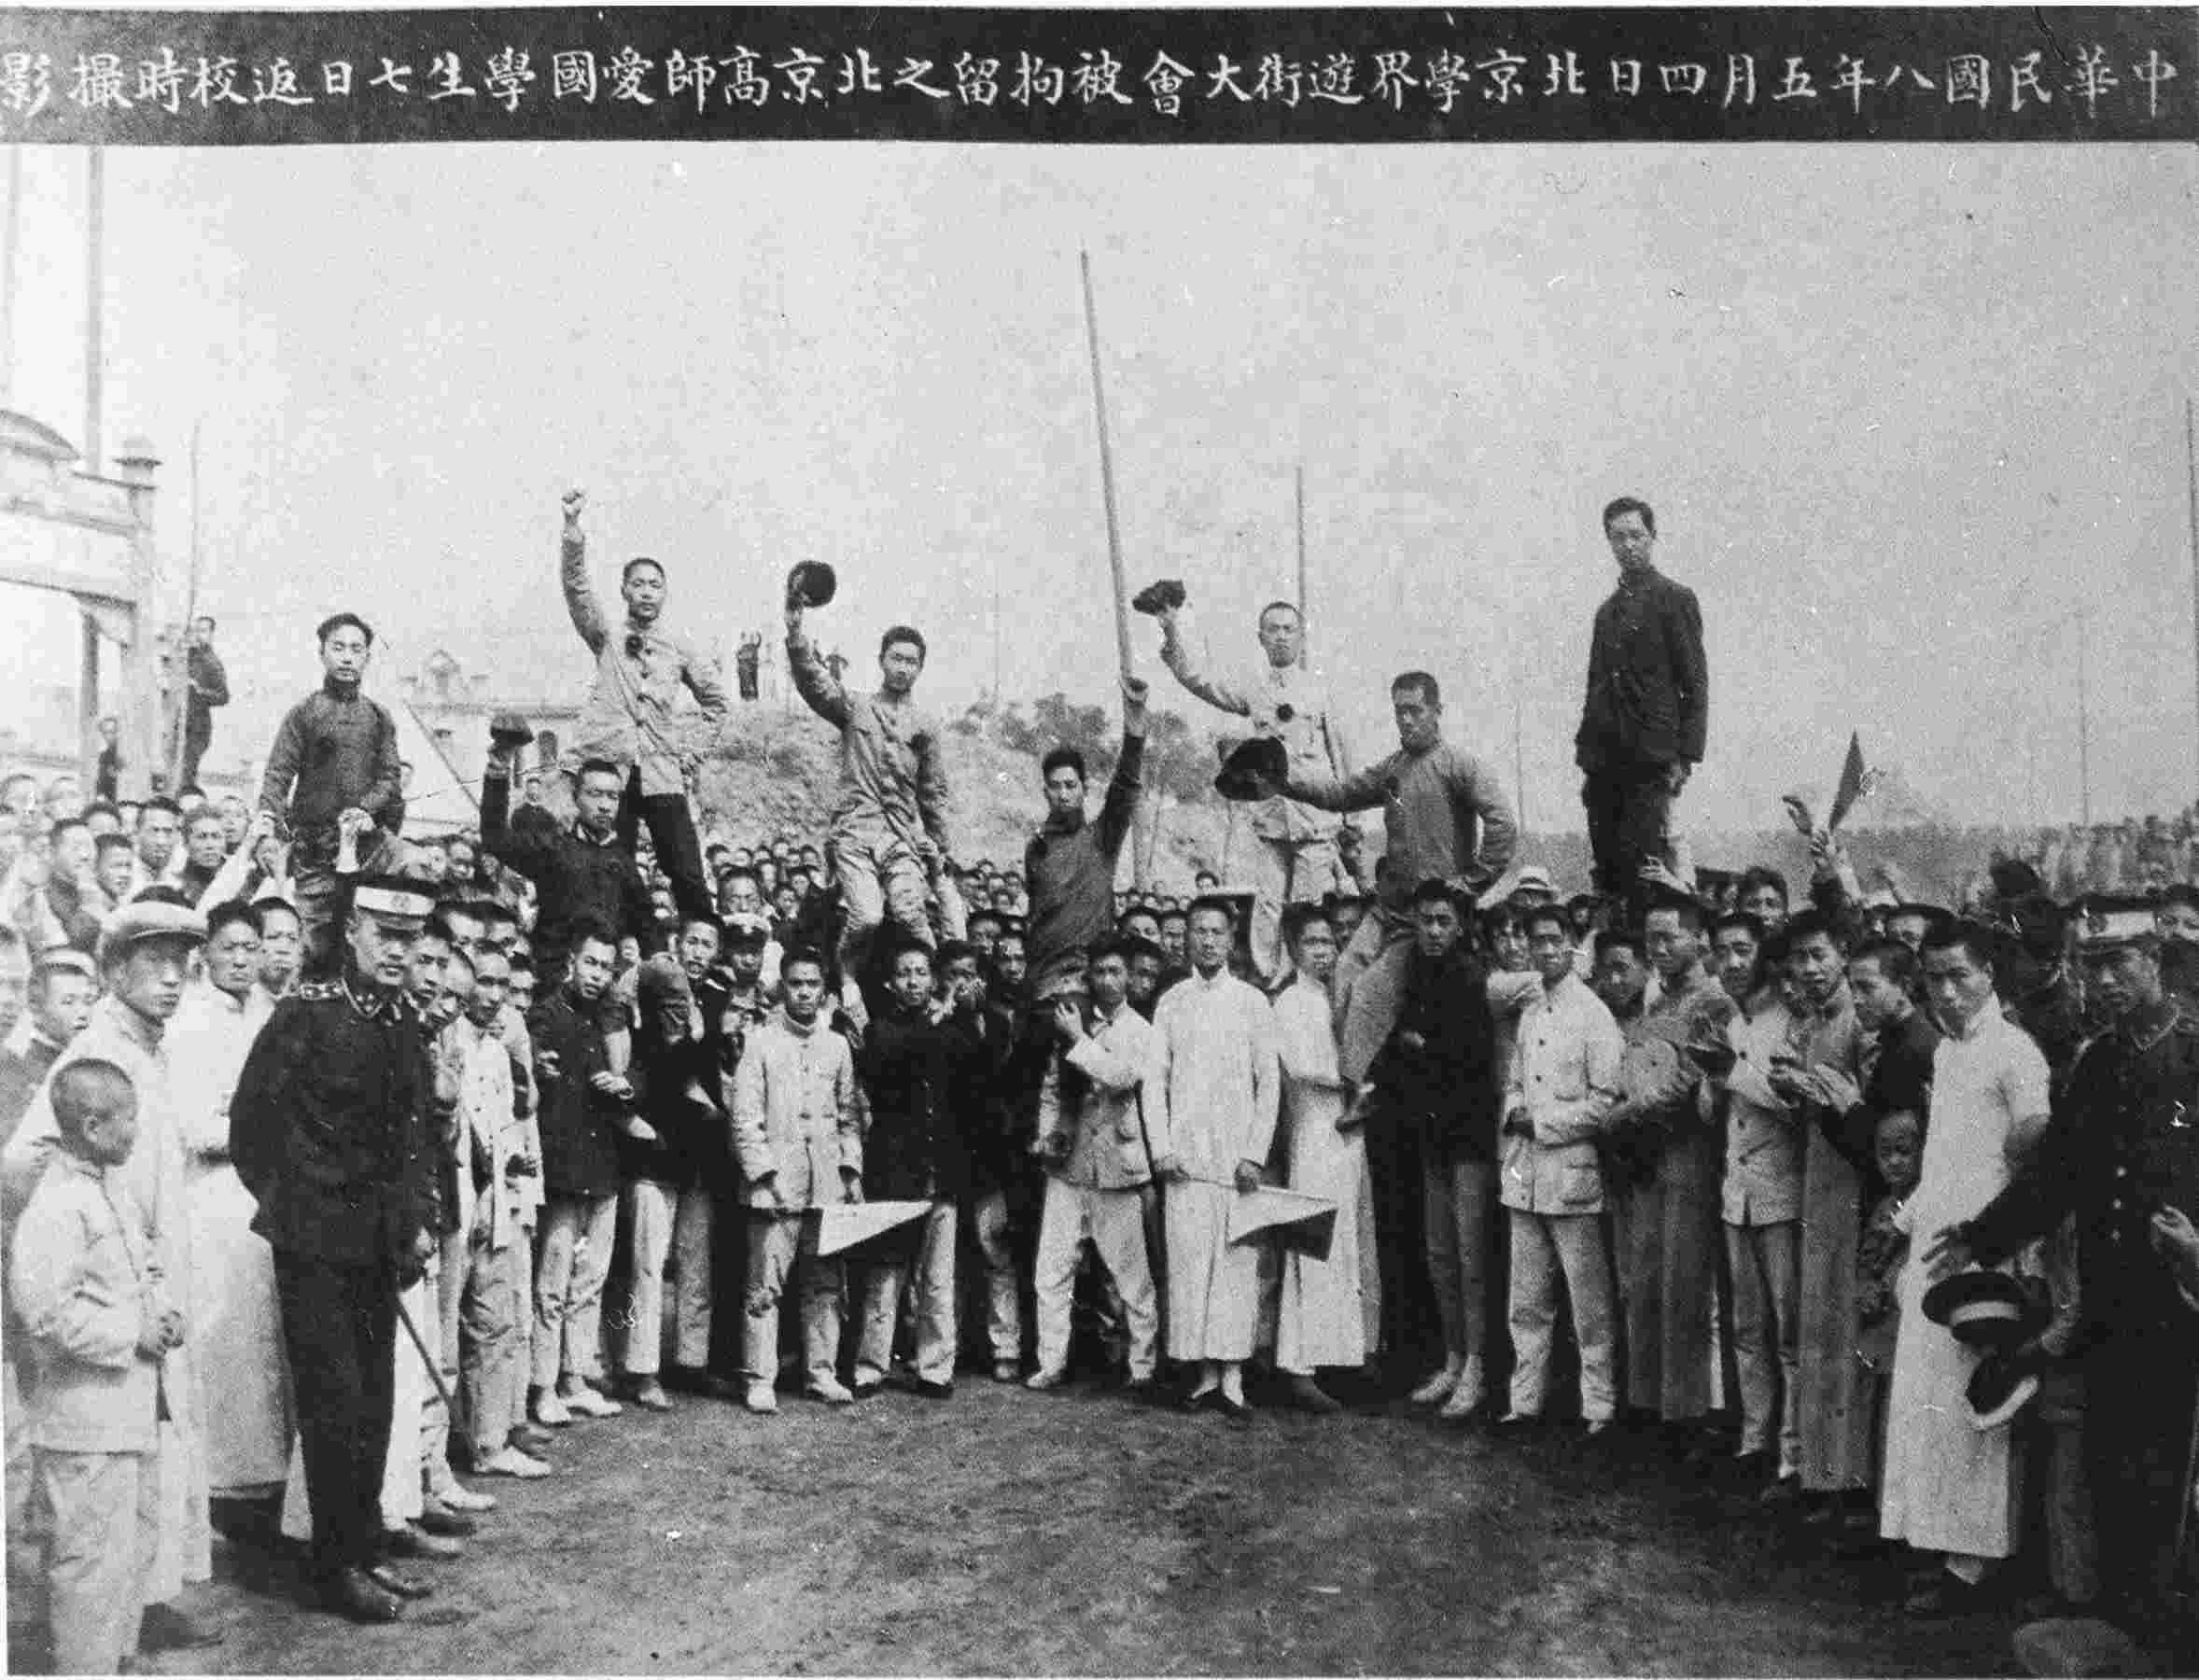
\includegraphics[scale=0.2]{Glava6/ZBi7nZhVeqE.jpg}
	%	\label{fig:scipion} % Unique label used for referencing the figure in-text\end{document}
	%	%\addcontentsline{toc}{figure}{Figure \ref{fig:placeholder}} % Uncomment to add the figure to the table of contents%----------------------------------------------------------------------------------------
	\caption{Пекинских студентов, только что выпущенных из под ареста за участие в несанкционированных акциях, встречает толпа}%	CHAPTER 2
\end{figure}

В начале июня в активную борьбу включились рабочие вместе с широкими средними городскими слоями и мелкой буржуазией. Главный центр движения при этом переместился из Пекина в самый развитый город страны - Шанхай, где забастовали 50—70 тысяч рабочих, а также почти все торговцы. Ну а далее подключилось составлявшее подавляющее большинство населения крестьянство. Под Аньхойцами ощутимо закачалась земля. Внезапно все вспомнили, что продолжает существовать некогда отодвинутый от реальных рычагов управления Гоминьдан. В итоге Пекинское правительство предпочло заявить о непризнании Версальского мирного договора, т.е. сделать популярный, хотя и чреватый опасностями, шаг во внешней политике, а не во внутренней. И ведь и его оказалось недостаточно – в решительность и патриотизм правительства всё равно никто не верил, и пришлось снять с постов ряд наиболее скомпрометировавших себя государственных деятелей. В конечном счёте Движение 4 мая всё же угасло. Наиболее умным из его лидеров было ясно, что любые попытки в одностороннем порядке оспорить решения Антанты при тех возможностях, которыми реально обладает Китай, обречены на провал. Демонстрации и митинги в Поднебесной успешно игнорировались, а любые более решительные действия вели к автоматической и очень жесткой конфронтации с Японией, которую в этом случае поддержат все крупные игроки. Внутри же страны не обладающие оружием и не имеющие четкой и жесткой организационной структуры группы не могли противостоять по большей части состоящим из военных кликам, оснащённым разнообразным вооружением и готовым его применять. Экономически одолеть режим клик тоже не получилось, так как часть буржуазии всё же предпочла продолжить сотрудничество с ними, получая их протекцию в условиях городских выступлений.

Но кое-что всё же вышло. Прежде всего, Движение 4 мая обозначило поворот во взглядах китайской интеллигенции: массовую переориентацию с традиционной культуры на вестернизацию. В частности же это выражалось в том, что прекратились попытки поиска глобального “своего пути” – в Поднебесной ускоренно укоренялись и развивались европейские направления политической мысли. В том числе стремительно распространялись марксизм, национализм европейского, научного типа, общее понимание того, что такое демократия, парламентаризм и тому подобное. Если в 1912 году Республика, президент, выборы были непривычными жупелами, то теперь превращение всего этого из ширмы в реально действующий механизм стало целями борьбы для целого ряда политических сил, которые позднее и придут к власти в Поднебесной – обновлённого Гоминьдана, КПК и некоторых других. Во-вторых, в попытке продемонстрировать жесткость и силу, способность решать масштабные задачи, стоящие перед Китаем, Аньхойская клика инициировала силовое занятие территории Монголии и лишение её автономии. На оперативно-тактическом уровне всё прошло достаточно легко – и китайские, и монгольские солдаты были плохо обучены и ещё хуже управлялись, но китайцы имели решающее превосходство в технике и вооружении. На дипломатическом фронте всё тоже прошло очень легко. Формально Монголия и так продолжала быть частью Китая. Некогда игравшая первую скрипку в делах региона Российская империя перестала существовать, а больше сохранность Кяхтинского соглашения 1915 года никто гарантировать и обеспечивать не собирался. Но стратегически вроде бы как успешная операция была крупной ошибкой. Если до 1919 о независимости в Монголии мечтала лишь довольно узкая прослойка верхов, то после прихода китайских солдат в качестве грабителей и агрессоров положение изменилось. Что ещё более важно, элиты упразднённой автономии не видя для себя перспектив, стали готовы пойти на союз с любыми, даже потенциально опасными силами. В итоге проход через Монголию частей Азиатской дивизии барона Унгерна в 1920, изначально имевший целью нанести удар в тыл красных в районе Бурятии, завершился установлением союза между свергнутым Богдо-ханом и русскими, по инициативе первого. В свою очередь этот альянс сумел выдворить китайские войска из окончательно обретшей уже полную независимость страны. Также Монголия оказалась тем самым вовлечена в общую орбиту Гражданской войны в России. К ней мы скоро и перейдём, добавив в китайской картине ещё один штрих.

Ещё одним и очень важным следствием Движения 4 мая стало ослабление Аньхойской клики в конкурентной борьбе. Играющая роль правительства, она получала и все шишки. Очень многие были недовольны тем положением, в котором находился Китай, при этом другие клики с удовольствием способствовали обращению народного гнева в правильном направлении. Прежде всего, Дуань Цижуй, не имевший с 10 октября 1918 никакой формальной должности, кроме своего генеральского звания, хотя и провёл в том же октябре 1918 своего кандидата в президенты – Сюй Шичана, начал постепенно терять влияние. На президента довольно активно давили и в какой-то момент он позволил себе весьма серьёзно подвести патрона. Тот, используя японские кредиты и союзнические военные поставки, за 1917-1918 год усилил верные лично ему войска Аньхойцев, и удар по Монголии, который наносился именно ими, должен был послужить ещё и акцией устрашения и пробой сил. В некотором роде получилось слишком хорошо – ранее колебавшаяся Фэнтяньская клика, базирующаяся на Манчжурию, перепугалась так сильно, что решительно переметнулась на сторону Чжилийцев – основных противников Дуань Цижуя. Тот приготовился действовать. И именно в этот момент президент под давлением политических противников (в виде блефа ссылавшихся ещё и на волю стран Антанты) отстраняет от дел генерала Сюй Шучжэна, главу монгольской экспедиции, ближайшего сподвижника лидера Аньхойцев. Незадолго до решающего столкновения Дуань Цижуй потерял лицо из-за действий слабосильных, и потому опасных союзников в лице президента и его команды, что сказалось и на боевом духе войск, и на намерениях неопределившихся командиров и группировок. Так или иначе, генералы Сюй и Дуань осудили действия Чжилийцев и Фэнтяньцев, к тому времени уже открыто и явно игнорировавших волю и требования прежних хозяев страны, и приготовились к войне. В начале июля 1920 года Аньхойская клика собрала 5 дивизий и 4 соединённые бригады и сформировала Армию национальной стабилизации . Главнокомандующим был назначен Дуань Цижуй. Чжилийская клика и союзники собрали одну дивизию и девять соединённых бригад и сформировали Армию подавления предателей, главнокомандующим передовой её части был назначен генерал У Пэйфу. 

\begin{figure}[h!tb] 
	\centering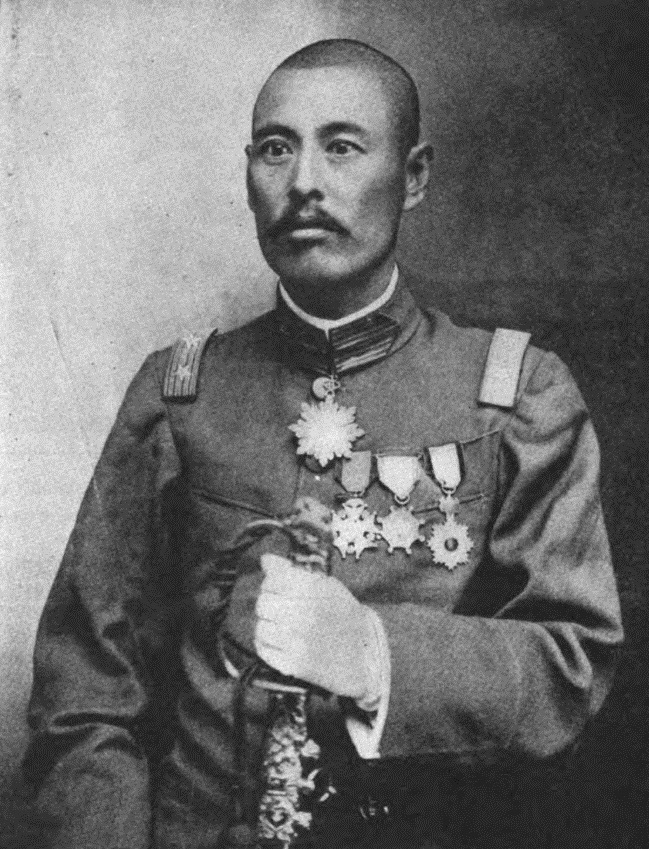
\includegraphics[scale=0.4]{Glava6/Iu72jXZsrns.jpg}
	%	\label{fig:scipion} % Unique label used for referencing the figure in-text\end{document}
	%	%\addcontentsline{toc}{figure}{Figure \ref{fig:placeholder}} % Uncomment to add the figure to the table of contents%----------------------------------------------------------------------------------------
	\caption{У Пэйфу — один из наиболее талантливых военачальников эры клик в Китае}%	CHAPTER 2
\end{figure}

Уже здесь можно наблюдать во многом сборный характер антианьхойских сил. В сочетании с тем, что уже первые удары, нанесённые 14 июля 1920 года аньхойской армией сразу на двух фронтах, заставили её врагов отступить, победа Дуань Цижуя виделась куда более вероятной. Так же оценивали ситуацию и японцы, а, кроме того, противники из клик Чжили и Фэнтянь в целом относились к Стране Восходящего солнца с куда большей опаской и скепсисом. Всё это, плюс затаённая надежда, что в лице лидера Аньхойской клики они получат, наконец, после его победы, человека, который сможет консолидировать Китай и целиком и без изъятий заставить его придерживаться достигнутых между странами договорённостей, привело к тому, что Япония пошла на открытую поддержку Дуаня. Разумеется, скромную, но символически очень важную. Через два дня после начала боёв, уже с помощью японских войск аньхойская армия заняла ещё ряд населённых пунктов, ранее контролировавшихся её противниками. Но на этом наступление аньхойских сил остановилось.

Совершенно неожиданно 17 июля У Пэйфу лично командуя западным фронтом Чжилийской армии, совершил дерзкий обход с фланга аньхойских сил и смог занять штаб-квартиру западного фронта врага. Результатом стало взятие в плен аньхойского главнокомандующего Цюй Тунфэна и многих офицеров, включая командующего Первой дивизией, что привело к нарушению командования и дезорганизации сил аньхойцев. Захватив Чжочжоу, У преследовал отступающую аньхойскую армию до самого Пекина. В процессе, как нетрудно догадаться, отход при слабом контроле командования, обратился в бегство. За исключением Пятнадцатой дивизии, весь западный фронт аньхойцев был разбит. Параллельно Фэнтяньская армия на вспомогательном направлении атаковала аньхойский восточный фронт. Узнав о прорыве линии западного фронта, командир восточного фронта, начальник штаба Сюй Шучжэн попросту струсил, сбежал в Пекин, оставив свои войска сдаваться чжили-фэнтяньской армии, что вскоре и произошло. Уже 19 июля Дуань Цижуй понял, что битва проиграна, и устранился от руководства Аньхойской кликой. 23 июля объединённые силы Чжили и Фэнтяня вошли в Пекин, после чего Аньхойская клика признала поражение и сдалась. Глобально это привело к тому, что наиболее сильный из лидеров, потенциально способный консолидировать в своих руках всю полноту власти во всех регионах страны, на долгое время выбыл из игры. Ослаблявший и изматывавший Китай режим борющихся клик сохранился. При этом наиболее успешно сотрудничавший с японцами человек, на которого в итоге открыто и гласно была сделана ставка, проиграл, и теперь Стране Восходящего солнца предстояло иметь дело с людьми, настроенными по отношению к ней гораздо хуже. Конечно, они не могли ни отменить 16 пунктов, ни радикально изменить роль и положение Японии в делах Поднебесной, но вот всячески ставить палки в колёса – это сколько угодно. Реализация конечных целей Страны Восходящего солнца в Китае опять сдвигалась по времени – и это очень серьёзно аукнется ей в ходе Вашингтонской конференции.

Иначе, но тоже достаточно неожиданно и драматично, развивались для японцев события в России.

Как мы помним, японская армия смогла достаточно легко занять обширные территории от Приморья и до Читы включительно, к началу 1919 года и количественно, и качественно японские войска были гораздо сильнее любых других на Дальнем Востоке и в Восточной Сибири. Были найдены готовые сотрудничать коллаборанты, вроде Семёнова, равно индифферентные к стратегическим целям красных и белых в Гражданской войне, не имеющие особых политических амбиций, при условии, что патронат японцев позволит им предаваться разгулу и грабежам. Постепенно развернулось и форсированное экономическое проникновение Японии на захваченные земли. Как правило, японцы действовали законным образом: они задешево скупали у собственников земельные участки, заводы и предприятия, пользуясь тем, что экономические связи с центром страны были разорваны, перипетии Гражданской войны резко повышали нестабильность и риски (особенно в случае победы большевиков), что в совокупности резко обесценивало прежде весьма выгодные активы и заставляло владельцев искать возможность поскорее продать их. Но в ряде случаев подданные императора Тайсё действовали и иными, куда более жесткими методами. Все лучшие рыболовные участки на тихоокеанском побережье были явочным порядком захвачены японскими рыбопромышленниками.

За многие материалы и продукты японцы, конечно, в первую очередь военные, вообще отказывались платить, просто их реквизируя. Массового террора не было, но любые подозрительные без церемоний и колебаний устранялись. Охотно солдаты Империи Восходящего солнца и грабили. Здесь примером послужит выдержка из Меморандума временного правительства — Приморской областной земской управы советнику японской дипломатической миссии в Сибири (март 1920 года): «1. …. 5. 18 января с. г. Василий Иванченко на разъезде Краевском арестован японским отрядом и расстрелян. 6. В июле 1919 г. японским отрядом отобрано имущество, принадлежавшее крестьянину д. Архангеловки, Успенской волости, Иманского уезда, Тарасу Коваленко, на 250 тыс. руб. 7. 8 февраля с. г. японским гарнизоном расстрелян в Черниговке, Никольск-Уссурийского уезда, ни в чем неповинный русский гр. Опанасенко. …. 9. 25 февраля с.г. японскими войсками убиты и расстреляны следующие лица: около разъезда Гедике ремонтный рабочий Федор Дворняк, на ст. Вяземской рабочий Иван Безкровный и путевой сторож 608 версты Гордей Цибунский с женою и двумя детьми….».

Действия интервентов вызвали сопротивление местного населения: только в Приамурье весной 1919 года действовало 20 партизанских отрядов, насчитывавших (по японским оценкам) 25 тысяч бойцов. Это означало, что надёжный контроль может сохраняться только при массовом присутствии армейских сил Японии. А вот с этим как раз были проблемы. Единственным поводом для сохранения фактической оккупации были решения объединённой межсоюзнической комиссии Антанты об интервенции, принятые ещё в ходе Первой Мировой. Теперь война окончилась. Существовало пользующееся поддержкой союзников (а по факту ими и поставленное) правительство Колчака - и вот у него в глубоком тылу, вне боевого контакта с красными, да и с кем-либо вообще, кроме партизан, находилась армия в 72 000 человек, не желавшая передавать в его руки административную власть и явным образом действующая не в его пользу, а сугубо исходя из собственных интересов. При этом строго формально Приморье продолжало относиться к Колчакии, что порой приводило к неприятным для одной и унизительной для другой стороны инцидентам, когда распоряжения Верховного Правителя, не соответствующие их видению и планам, отменялись японцами.

Империя Восходящего солнца легко могла бы безо всяких экивоков установить режим оккупации и отделаться от Колчака и всех прочих, если бы кроме её войск на очерченной выше территории не было других антантовских контингетов. Но они были - гораздо более слабые, но заставляющие японцев увязывать все свои действия с общесоюзнической повесткой. И с ними поделать было нельзя ничего - их нельзя было атаковать, нельзя было вытеснить, нельзя купить или принудить к сотрудничеству. В итоге в случае победы в Гражданской войне Колчака, японцам пришлось бы просто уйти вместе с остальными. Конечно, они получили бы экономический доступ к российским ресурсам - на Колчака ставили и помогали ему не для того, чтобы он повёл подлинно самостоятельную экономическую политику, но строго на равных основаниях с прочими интересантами. Прямая же конкуренция с товарами и капиталами США в Приморье... Одним словом, особенно выигрышным такое развитие событий в Токио счесть никак не могли.

Много выгоднее была бы затяжка Гражданской войны, такая ситуация, при которой тот же Колчак сам, нуждаясь в помощи японцев - чисто военной, или в форме поставок снаряжения и материалов, в той или иной форме одобрил бы их пребывание в России, оформил его двусторонним межгосударственным договором, что отвязало бы Японию от Антантовской упряжки, переведя ситуацию на рельсы, близкие к тем, по которым она катилась в Китае. Частично этот план уже работал - Верховный Правитель был вынужден подписать ряд договоров о предоставлении японцам концессий, но на большее он пока не шёл. Японцы, чтобы не дразнить гусей в лице США и остальных, не напирали, полагая, что время и шансы у них ещё есть. И тут...

В октябре 1919 года было остановлено самое опасное, по существу – единственное действительно угрожавшее существованию Советской России, наступление белых сил – удар ВСЮР Деникина на Москву. Не место и не время распространяться на тему, почему так случилось - суть в том, что с этого момента в Гражданской войне в России наступил окончательный перелом. Белые силы как потерпели крах в попытке овладеть столицей, так и не смогли соединиться летом 1919, несмотря на кратковременное падение стратегически важного Царицына, который большевикам удалось оперативно отбить, так что РККА сохранила возможность манёвра силами против разных фронтов и их концентрации. Малочисленность, растянутость коммуникаций, угроза обхода и окружения в районе Орла-Брянска наиболее боеспособных частей ВСЮР заставила Деникина предпринять зимой 1919-1920 стремительное отступление с целью сократить фронт и приблизить его к социально-экономической базе движения на Кубани. Белой армии в общем и целом удалось избежать прямого военного разгрома, но объём оставленной и перешедшей в руки красных территории с населением и промышленными предприятиями, а были отданы такие города, как Харьков, Киев, города Донбасса, Ростов-на-Дону, сделал положение белых стратегически безнадёжно проигранным, что и продемонстрирует уже 1920-й.

Но это - Европейская Россия. В Сибири же гораздо менее даровитый в военном отношении Колчак уже в ноябре 1919 получил фатальный удар, заставивший его начать так называемый Великий Сибирский Ледяной Поход (Да, только и именно так, Всё С Большой Буквы!), а по факту стремительное отступление, граничащее с бегством, на восток. 4 ноября 1919 - сразу после того, как стабилизировалось положение в боях с ВСЮР и появилась возможность впервые за долгое время подбросить подкрепления Восточному фронту, 3-я (командующий М.С. Матиясевич) и 5-я (командующий М.Н. Тухачевский) армии РККА переходят в наступление, начиная Омскую операцию. 

\begin{figure}[h!tb] 
	\centering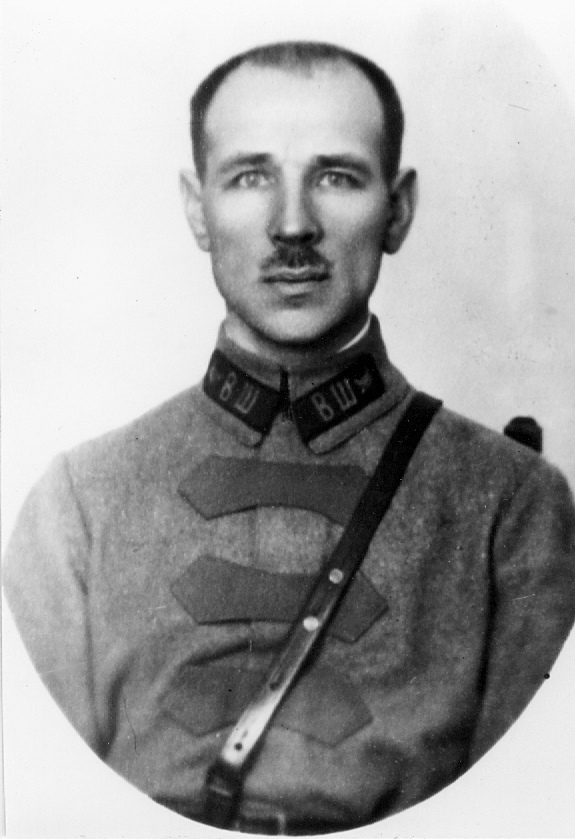
\includegraphics[scale=0.7]{Glava6/IWdsdZ-_1jk.jpg}
	%	\label{fig:scipion} % Unique label used for referencing the figure in-text\end{document}
	%	%\addcontentsline{toc}{figure}{Figure \ref{fig:placeholder}} % Uncomment to add the figure to the table of contents%----------------------------------------------------------------------------------------
	\caption{Командарм Матиясевич}%	CHAPTER 2
\end{figure}

5-я армия РККА наступала вдоль Транссиба, а 3-я армия вдоль железной дороги Ишим — Омск. Одновременно 59-я стрелковая дивизия и 13-я кавалерийская дивизия красных развернули наступление на Кокчетав и Атбасар против войск атамана Дутова. А уже 13 ноября из Омска выехали пять поездов, составлявших личный штаб Верховного Правителя адмирала Колчака, один из них с золотым запасом. Назначенный 4 ноября главнокомандующим К.В. Сахаров, который должен был организовать оборону столицы колчаковского государства, со своим штабом выехал из Омска на восток 14 ноября.

После фактического драпа командования боевой дух колчаковцев был подорван: в ночь с 13 на 14 ноября 1919 года 242-й Волжский стрелковый полк РККА скрытно переправился по льду на восточный берег Иртыша, красноармейцы без единого выстрела заняли ж/д станцию Омск, здания вокзала и к утру попросту разоружили 7000 белых солдат и офицеров, находившихся в эшелонах. Утром 14 ноября ими был взят в плен белогвардейский генерал Римский-Корсаков, прибывший на место службы - ему просто оказалось уже нечем командовать. Красные войска почти не встречая сопротивления подошли непосредственно к Омску и 15 ноября без боя заняли город. В целом взятие Омска было настолько неожиданным, что колчаковские учреждения были захвачены при нормальном режиме работы.

2-я и 3-я армия белых отступили к Новониколаевску и Томску. 14 декабря пал Новониколаевск (ныне Новосибирск). После взятия Новониколаевска сопротивление белых вдоль Транссиба было практически парализовано, через 10 дней они сдали красным важнейшие административные центры: Томск (без боя), Кузнецк, Мариинск и Красноярск. Держава Верховного Правителя сжималась, как шагреневая кожа. Колчак утратил полезность для тех, кто его двигал, кто на него ставил, и кто с ним проиграл. Свою роль сыграли и попытки адмирала сохранить контроль над золотым запасом и другими ценностями. Едва ли стоит удивляться тому, что Колчак в итоге был арестован и выдан чехословаками – т.е. явно не без ведома контролировавших их ведущих держав Антанты.

Любопытно, что в последний момент “тонущего” адмирала попытались перехватить японцы: акт передачи арестованного Верховного правителя был составлен 15 января в 21:55, а утром того же дня командующий японскими войсками Иркутска полковник Фукуда, узнав о прибытии в город поезда с Колчаком, обратился к Яну Сыровому - командиру чехословаков с просьбой передать пленника под охрану японского батальона, на что получил ответ, что Колчак уже выдан повстанцам. Зачем Японии был нужен всё потерявший Колчак? Причина одна - сохраняя статус Верховного Правителя, он ещё мог легитимизировать японские захваты, причём, оказавшись в полностью зависимом от доброй воли Фукуды и его командиров положении, почти наверняка сделал бы это почти без торга. Можно себе представить, как кусали локти в Токио, когда сообразили, что опоздали буквально на несколько часов!

Разгром Колчака в конце 1919 — начале 1920 года стал рубежным моментом. С этого времени страны Антанты уже не рассчитывали на уничтожение Советской России и крах большевизма в краткосрочной перспективе. Было ясно, что без радикального увеличения своей собственной вовлеченности в конфликт, белое дело его зарубежным друзьям уже не спасти. Для всех, кроме японцев, после этого интервенция потеряла смысл, став просто затратной, небезопасной и политически неудобной в силу роста влияния левых движений и партий. Можно ещё было вывезти кое-какие ресурсы и ценности, но глобально ловить в России стало нечего. США и другие державы были вынуждены начать вывод войск. Американцы в основном произвели его в январе-марте 1920, завершив его к апрелю (впрочем, американские корабли оставались во Владивостоке до 1922 года), до июля 1920 вывели свои войска как непосредственно с территории РСФСР, так и из Закавказья, Англия и доминионы Британской империи.

Однако численность японских войск не только не упала, но продолжала увеличиваться. Наступал момент истины - с одной стороны непосредственно на месте не осталось никого, кто мог бы сдержать японцев, или помешать им, с другой очень скоро державы Антанты начнут настоятельно интересоваться, что именно задерживает силы Империи Восходящего солнца в России. Существовало две возможности. Первая - всё же добиться подписания комплекса документов, который узаконил бы как минимум пребывание японских войск, а как максимум давал бы Японии вещественные и закреплённые юридически права и привилегии. Но кто мог бы это сделать?

С точки зрения формальных полномочий в Белом движении наступил полный бардак. Колчак, ещё будучи облечённым властью, декларировал, что в случае тяжкой болезни или смерти Верховного Правителя, а также на случай отказа его от звания Верховного Правителя или долговременного его отсутствия, полномочия высшей власти будут переданы Главнокомандующему Вооружёнными силами на Юге России генерал-лейтенанту Деникину. 24-го июня 1919 Деникин был назначен заместителем Главкома вооруженных сил. Впрочем, всё это было скорее способом подсластить командиру ВСЮР пилюлю формального подчинения Колчаку, тем более, что реальной связи и единства действий между Сибирским и Южным очагом Белого движения так никогда и не возникло. Непосредственно перед низложением - за 10 дней до него, 4 января 1920 года Колчак издал в Нижнеудинске указ, которым «ввиду предрешения… вопроса о передаче верховной всероссийской власти Главнокомандующему Вооружёнными силами на Юге России генерал-лейтенанту Деникину, впредь до получения его указаний, в целях сохранения на нашей Российской Восточной Окраине оплота государственности на началах неразрывного единства со всей Россией» предоставлял «всю полноту военной и гражданской власти на всей территории Российской Восточной Окраины, объединённой российской верховной властью», генерал-лейтенанту Г. М. Семёнову. И понимайте это как знаете! Нельзя исключать, что такое вот возвышение Семёнова было попыткой заручиться поддержкой Японии, с которой он был тесно связан, но своевременно всё проделать ни той, ни другой заинтересованной стороне не удалось. В довершении всего, так и не приняв на себя полномочий Верховного Правителя (а в реальности плевав на них) Деникин 4 апреля 1920 уходит с поста командира ВСЮР. На итог у японцев оставался Семёнов - вполне верный, готовый подписать любые бумаги, но и большевикам, и Антанте, и даже занявшему место Деникина Врангелю ничего не стоило при желании дезавуировать в дальнейшем любые его решения.

Второй же возможностью было вступление в бой со стремительно приближавшимися силами большевиков. Само по себе свержение большевизма интересовало Японию образца 1919-1920 постольку поскольку. Тем более, что Гражданская война уже практически окончилась - к концу марта 1920, разбитые на Кубани, части ВСЮР начали процесс эвакуации в Крым и концентрации там. Большая часть исторической России контролировалось Советским правительством, что возрождало все прежние сложности, о которых мы писали раньше применительно к возможности новой Русско-японской войны и того, почему в самой Японии этот вариант всерьёз не рассматривался. Было совершенно непонятно, как нанести красным такого масштаба поражение, чтобы они оказались вынуждены прекратить борьбу и принять навязываемые японцами условия. Нет, Японии была совершенно не нужна большая война против РСФСР - нужна была такая, которая не позволит РККА дойти до Тихого океана, а главное - не позволит США и другим странам Антанты обвинять Японию в захватнических планах. Какие захваты? Только борьба с большевистской заразой. Но здесь было две проблемы. Первая - чересчур выдающееся в глубину Сибири расположение передовых японских сил. Если прежде, когда кроме партизан никто им не угрожал, это было нормально и даже выгодно, то теперь ситуация переменилась. Красные вполне могли отрезать находящиеся в Прибайкалье японские части от линий снабжения, окружить и уничтожить их. Построить же плотный многокилометровый фронт в этой части Сибири было невероятно трудно и дорого. Нужно было отойти. Но как? Сам по себе отход уже был в известной мере потерей лица. И, что важнее, ни в коем случае нельзя было создавать впечатления "кооперативной игры", тайных договорённостей с большевиками.

И вот в этот момент появляется 6 апреля 1920 Дальневосточная Республика - совершенно гениальный ход советской дипломатии. Формально не являющееся ни большевистским, ни даже советским государство, со всеми атрибутами парламентской демократии, независимое по всем формальным же критериям от Москвы, оно резко увеличивало поле для манёвра и для РСФСР, и для Токио. Японцам создание ДВР дало возможность приобрести партнёра для переговоров, причём такого, отношения с которым никак не регулировались и не регламентировались решениями Антанты и положениями Версаля, позволило вновь, как бы борясь с большевиками, иметь между ними и собою буфер, как при Колчаке, наконец, надежду со временем добиться превращения временного в долгосрочное - созданная сугубо "под задачу" ДВР, тем не менее, юридически вывела из состава РСФСР Дальний Восток и Приморье, чем можно было со временем воспользоваться. Благо у Японии уже был опыт превращения некогда вассальной Китаю Кореи сперва в своего вассала, а затем - и в свою колонию. Для Советского правительства ДВР давала возможность избежать прямых и серьёзных военных столкновений с Японией, окончательно добить у них под носом своих врагов в Сибири, параллельно решая ключевые военные задачи в Европе - в Крыму и в Польше. Ну а в конечном счёте обвести японцев вокруг пальца, ликвидировав ДВР в тот момент, когда она утратит свою полезность. В целом это чем-то напоминает современные ДНР и ЛНР и вообще практику прокси войн и прокси переговоров, только вот РСФСР и ДВР действовали гораздо решительнее и умелее, чем нынешние российские власти.

\begin{figure}[h!tb] 
	\centering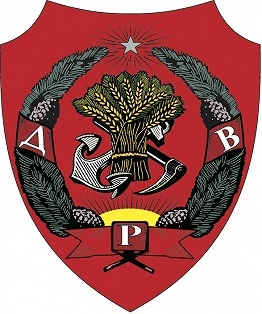
\includegraphics[scale=0.6]{Glava6/njN-LQYB2jI.jpg}
	%	\label{fig:scipion} % Unique label used for referencing the figure in-text\end{document}
	%	%\addcontentsline{toc}{figure}{Figure \ref{fig:placeholder}} % Uncomment to add the figure to the table of contents%----------------------------------------------------------------------------------------
	\caption{Герб ДВР}%	CHAPTER 2
\end{figure}

Ну а теперь по хронологии. 6 апреля 1920 ДВР появляется как ещё по сути своей виртуальное образование - оно не контролирует и 10\% территории, на которую претендует. Для конспирации реально задействуются несоветские элементы в управленческих кадрах менее приоритетных министерств и ведомств. Несколько затягивается и процедура признания - Советская Россия официально признала ДВР 14 мая 1920 года, в то же время предоставив ей с самого начала финансовую, дипломатическую, кадровую, хозяйственную и военную помощь. Это позволило Москве контролировать внутреннюю и внешнюю политику ДВР и создать Народно-революционную армию (НРА) на базе красных дивизий. И в этот же день, 14-го, командующий японскими войсками на Дальнем Востоке генерал Юи Мицуэ объявил о согласии вести переговоры с ДВР. 

\begin{figure}[h!tb] 
	\centering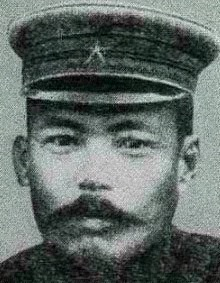
\includegraphics[scale=0.6]{Glava6/ewTaUGtiF2w.jpg}
	%	\label{fig:scipion} % Unique label used for referencing the figure in-text\end{document}
	%	%\addcontentsline{toc}{figure}{Figure \ref{fig:placeholder}} % Uncomment to add the figure to the table of contents%----------------------------------------------------------------------------------------
	\caption{Генерал Юи Мицуэ}%	CHAPTER 2
\end{figure}

24 мая на станции Гонгота начались официальные переговоры ДВР и японского командования. Как предварительное условие было принято, что «НРА и экспедиционные силы японской империи не вели и не ведут войну, случаи столкновения, вызванные взаимным непониманием, должны рассматриваться как печальные недоразумения». Первоначально японцы решили, так сказать, взять на испуг и предложили создать западнее Читы нейтральную зону, которая бы отделила части НРА от японских и семёновских войск.

ДВР ответила весьма решительно, предъявив ещё более неисполнимые требования:

Перемирие на всех фронтах, включая партизанские,

Отказ японцев от поддержки атамана Семёнова,

Эвакуация японцев с территории ДВР (т.е. полное очищение Дальнего Востока и Приморья, на которые она претендовала).

Причём ход со стороны ДВР в целом был сильнее. Понятно, что никто и не подумал бы принимать её условия и уходить, но японцы должны были придумать и официально огласить повод, по которому они остаются. В конечном счете, японцы отказались от эвакуации войск, ссылаясь на угрозу Корее и Маньчжурии, потребовали признать Семёнова за равноправную сторону при переговорах об объединении дальневосточных областных властей, и стремились ограничиться лишь соглашением с ДВР, чтобы разгромить восточно-забайкальских партизан. В начале июня переговоры прервались из-за отказа делегации ДВР признать экстренно созданное при японской поддержке «правительство Российской Восточной окраины» как равноправную сторону на будущих переговорах об объединении областных правительств. В целом ДВР тянула время - летом 1920 в самом разгаре была Советско-Польская война, в которой наметился к июлю стратегический перелом - наступавшие поляки были разгромлены, фронт покатился к Варшаве. Японцы же попытались сепаратным образом достигнуть договорённостей с угрожавшими их тылам партизанами: в результате переговоров на разъезде Алеур 2 июля было заключено перемирие между японскими войсками и партизанскими силами в районе правого берега реки Шилка, а 10 июля — для левого берега. Наконец, 3 июля японское командование опубликовало декларацию об эвакуации своих войск из Забайкалья, приглашая ДВР к возобновлению переговоров об условиях этого процесса. 10 июля делегации сторон вновь встретились на станции Гонгота. 16 июля стороны обменялись нотами, в которых, идя на уступки японцам, ДВР брала на себя обязательство, что «буферное государство не положит коммунизм в основу своей социальной системы», что не допустит на свою территорию советские войска и, что особенно важно, гарантирует «в сфере своего влияния личную неприкосновенность японских граждан и уважение прав» - в том числе и прав на приобретённую в ходе оккупации собственность. 17 июля было подписано соглашение о нейтральной зоне от станции Гонгота до станции Сохондо с границей по меридиану 113 градусов 30 минут восточной долготы. 25 июля 1920 года началась эвакуация японских войск из Забайкалья, окончившаяся 15 октября.

За это время успела фактически окончиться Советско-польская - хотя официально мир будет заключен 18 марта 1921, реально боевые действия в основном завершились к октябрю 1920. Не сумев сломить поляков и пробиться к бурлящим Германии и Венгрии, руководство РСФСР сконцентрировалось на решении проблемы оставшихся последствий Гражданской на территории России. В ноябре 1920 будет успешно проштурмован Крым. И параллельно на Дальнем Востоке сразу же после ухода японцев был атакован оставшийся без их протекции Семёнов. Под давлением превосходящих сил Народно-революционной армии ДВР 22 октября 1920 года семёновцы оставили Читу и отступили из Забайкалья, причём не в Приморье к японцам, а в Маньчжурию - ещё одно явное следствие соглашения. Самому Семёнову пришлось спасаться из Читы на аэроплане, причём фактически он бросил при этом армию, которая с этого времени почти перестала подчиняться резко утратившему авторитет командиру, окончательно превратившись в банду. Победа над белыми была достигнута.

Тем не менее, к концу 1920 японцы ощущали себя в Приморье весьма уверенно. С чисто военной точки зрения Япония имела крупные и уже не висящие в воздухе, а имеющие крепкий и оборудованный тыл, не столь далеко располагающиеся и от домашних баз силы, готовые отразить удар как частей НРА Дальневосточной Республики – полностью, с перспективой перейти в контрнаступление, так и РККА – вплоть до прибытия подкреплений. Для международного прикрытия своих действий существовал совершенно марионеточный, хотя и не очень респектабельный, из-за чего его в конечном итоге было решено слить, режим Семёнова и его головорезов, а главное – перспективы дальнейших переговоров с ДВР, её постепенного отдаления от РСФСР. За счёт чего? За счёт включения в неё областей, где сохранялся преимущественно японский контроль над экономическими активами, имелась готовая исполнять волю азиатских хозяев прослойка элиты – ну и конечно, на своём месте оставалась армия. С дозволения Японии после того, как окончательный крах потерпел Семёнов, на состоявшейся в Чите 28 октября — 11 ноября 1920 конференции представители трёх областных правительств (Забайкальской, Амурской, Приморской областей /в том числе, Камчатка и Чукотка/) законодательно оформили объединение в рамках Дальневосточной республики. Теперь доля японского в ней сравнялась с долей российско-советского, и Империя Восходящего солнца рассчитывала, что с течением времени – только дайте срок, она получит перевес и возьмёт верх.

Вот только времени этого у Японии не оказалось. Дипломатия РСФСР более точно просчитала общую международную ситуацию. Ключевой ошибкой Японии было то, что она полагала все последствия Первой мировой окончательно урегулированными в ходе Парижской конференции и оформленной не подлежащими пересмотру положениями Версаля. Кроме того, вывод войск всех прочих союзников из России и образование нового субъекта международного права – ДВР, по которому в рамках Антанты не было (да и быть не могло) никаких соглашений, переводил русскую политику Японии в удобное для неё русло совершенно независимых отношений. Да и вообще с концом войны Япония переставала быть частью каких-либо объединений и блоков, кроме Англо-японского союза, тем самым могла проводить независимую политическую линию, ни на кого более не оглядываясь.

Всё это оказалось опасными заблуждениями. За 1914-1920 годы Япония приобрела очень многое, а главное – поразительно малой ценой. И это вызывало зависть и опасения у ряда других игроков, ключевым из которых были Соединённые Штаты. Американцев интересовали два вопроса – экономическая выгода и безопасность. Выгодным для Штатов, имевших могучую промышленность и державших после ПМВ в должниках половину мира, было создание максимально широкой и стабильной зоны свободной торговли. В идеале таможенные барьеры, протекционистские тарифы и прочие ограничения должны были быть уничтожены по всему Земному шару. США – пока ещё в мягкой форме, начинают подрывать прежнюю экономическую систему, где ключевой линией отношений были отношения метрополия-колонии. И, в любом случае, американцы совершенно не были намерены упускать такой огромный рынок, как Китай. В конце 1920 они выступили инициаторами создания международного банковского консорциума в Китае, где первую скрипку играл, разумеется, американский капитал. В целом США, господствуя во всех отношениях в Центральной и Латинской Америке, владея Филиппинами, намеревались сделать Тихий океан своей вотчиной.

И – здесь мы переходим к вопросу безопасности – единственной страной в регионе, обладающей крупным военным флотом, была Япония. Причём она этот флот последовательно и быстро усиливала. Если уставшие от войны европейцы неуклонно снижали военные расходы, то Страна Восходящего солнца их наращивала. Ко всему на Японию было очень сложно нажать мягко: её нельзя было шантажировать долгами – по той простой причине, что долгов не было, невозможно было угрожать и вложенным в американские корпорации капиталам – они тоже отсутствовали. Тем не менее, японцам постарались намекнуть на то, что чрезмерно быстрое и активное усиление без одобрения и консультаций с США может привести её к неприятным последствиям. В 1920 году США вводят дискриминационные в отношении выходцев из Японии иммиграционные законы – явный недружественный и привлекающий внимание жест. В Токио, конечно же, его заметили, поворчали, но, в общем и целом, ничего не предприняли. И вот тогда тучи стали сгущаться очень быстро. Весьма вероятно, что последней каплей стала чрезвычайно активная политика Японии в России – вопреки, достигнутым, судя по всему, негласным договорённостям с маркизом Сайондзи в Париже. 14 декабря 1920 сенатор Бора внёс в Конгресс США предложение о созыве конференции по ограничению морских вооружений. 24 февраля 1921 это предложение было включено в виде поправки к морскому биллю, принятому Конгрессом. Параллельно в феврале 1921 канадский премьер Мейген выдвинул предложение о заключении договора четырёх держав (США, Великобритании, Японии и Франции) взамен англо-японского союзного договора. 

\begin{figure}[h!tb] 
	\centering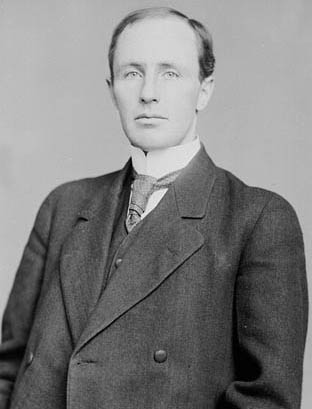
\includegraphics[scale=0.8]{Glava6/ePnbL90bYbw.jpg}
	%	\label{fig:scipion} % Unique label used for referencing the figure in-text\end{document}
	%	%\addcontentsline{toc}{figure}{Figure \ref{fig:placeholder}} % Uncomment to add the figure to the table of contents%----------------------------------------------------------------------------------------
	\caption{Артур Мэйген — премьер-министр Канады. Лично лояльный к метрополии, был вынужден предпринимать шаги, с целью несколько унять своих политических противников, утверждающих, что Англия слишком мало делает для Канады и её безопасности}%	CHAPTER 2
\end{figure}

План Мейгена обсуждался на Британской имперской конференции летом 1921. Наконец, 5 июля 1921, сразу после конференции, английский министр иностранных дел лорд Керзон в переговорах с послом США Харвеем предложил включить дальневосточные и тихоокеанские вопросы в повестку дня проектируемой конференции, тем самым согласившись с американским проектом. Фактически уже в этот момент Британия “сдала” своего союзника и судьба Японии была по большей части решена. 10 июля 1921 государственный секретарь США Юз сделал публичное заявление с предложением созвать конференцию в Вашингтоне. Державам было послано официальное приглашение от имени правительства США.

\begin{figure}[h!tb] 
	\centering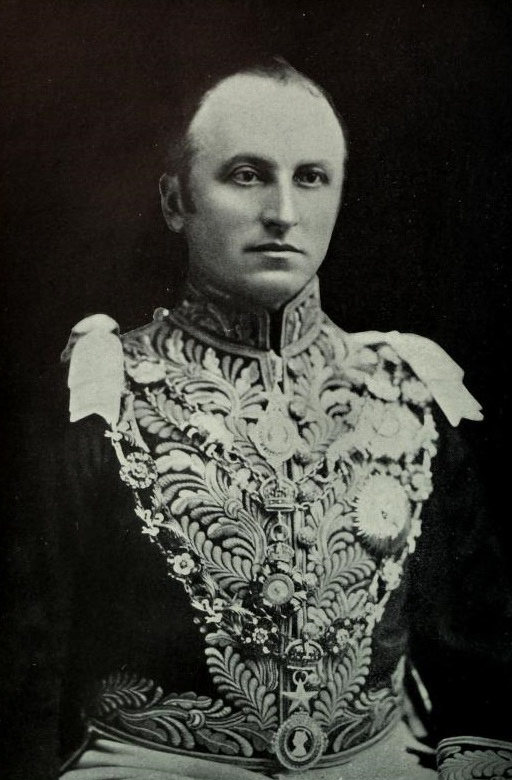
\includegraphics[scale=0.4]{Glava6/ml4n5yxZ3No.jpg}
	%	\label{fig:scipion} % Unique label used for referencing the figure in-text\end{document}
	%	%\addcontentsline{toc}{figure}{Figure \ref{fig:placeholder}} % Uncomment to add the figure to the table of contents%----------------------------------------------------------------------------------------
	\caption{Лорд Керзон}%	CHAPTER 2
\end{figure}

В Японии отнеслись к конференции отрицательно, сознавая, что сам её формат не сулит японцам ничего хорошего. О ней даже высказывались порой в таком ключе, что "Японию привлекают к суду англо-американского трибунала". Изначально японцы попросту попытались добиться её отмены, выступая в том духе, что для решения планируемых вопросов нет необходимости организовывать некую масштабную коллегию, поневоле вызывающую ассоциацию с Парижской конференцией. По флотам предлагалось отдельно от других государств и проблем договориться тем, кто их имел – США, Англии и Японии. Ранее же рассмотренные вопросы – в частности по Китаю, японцы вновь поднимать не хотели. Все попытки как-либо откорректировать состав, статус и повестку конференции были решительно пресечены американской дипломатией.

В то же время угрозу и в целом значимость события считали куда меньшими, чем у Парижской конференции. Япония была по-прежнему убеждена, что теперь могут происходить лишь небольшие изменения в уже начерченном плане поствоенного миропорядка. Это отношение ясно видно и по составу делегации Империи Восходящего солнца. В Версале договор от её имени подписывал человек, облеченный, вероятно, наибольшей реальной властью в Японии, один из трёх остававшихся гэнро, выражавший их коллективную волю, человек больших личных дарований и опыта. В Вашингтон же поехал, помимо сугубо вспомогательных кадров, лишь морской министр Като Томосабуро. 

\begin{figure}[h!tb] 
	\centering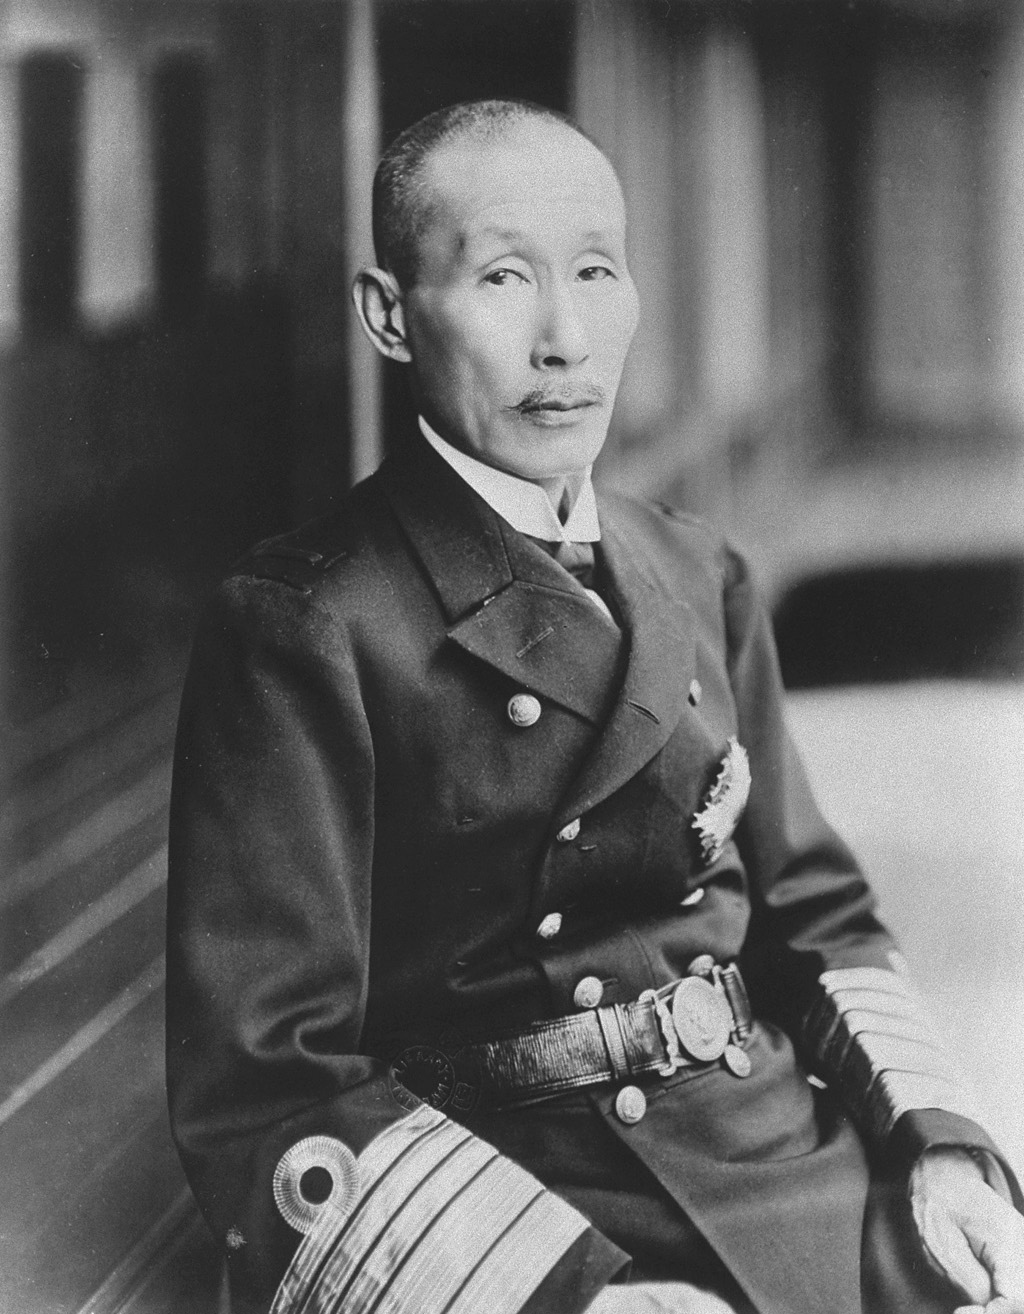
\includegraphics[scale=0.3]{Glava6/EVMZtG3m7CE.jpg}
	%	\label{fig:scipion} % Unique label used for referencing the figure in-text\end{document}
	%	%\addcontentsline{toc}{figure}{Figure \ref{fig:placeholder}} % Uncomment to add the figure to the table of contents%----------------------------------------------------------------------------------------
	\caption{Като Томосабуро}%	CHAPTER 2
\end{figure}

Некогда бывший начальником штаба великого Того – в том числе во время Цусимского сражения, это был храбрый и толковый моряк, но ни дипломатией, ни вообще политикой он никогда прежде не занимался – иными словами, те, кто его направлял, полагали, что конференция в самом деле в первую очередь будет посвящена морским вооружениям – вопросу, прежде не затронутому в Версале – только в отношении побеждённых стран и ограничения их вооружённых сил в целом. Кроме Като в числе руководителей японской делегации был Кидзюро Сидэхара – профессиональный дипломат, однако, лишь в 1919 году назначенный послом в Соединённые Штаты и не имевший там особенного влияния и связей. Ни министра иностранных дел, ни премьера Хара Такаси, ни, тем более, кого-то из гэнро. В итоге Япония явно не вполне готовой сделала шаг в пасть звёздно-полосатому тигру. Шаг к страшному поражению и чудовищному унижению.

\begin{figure}[h!tb] 
	\centering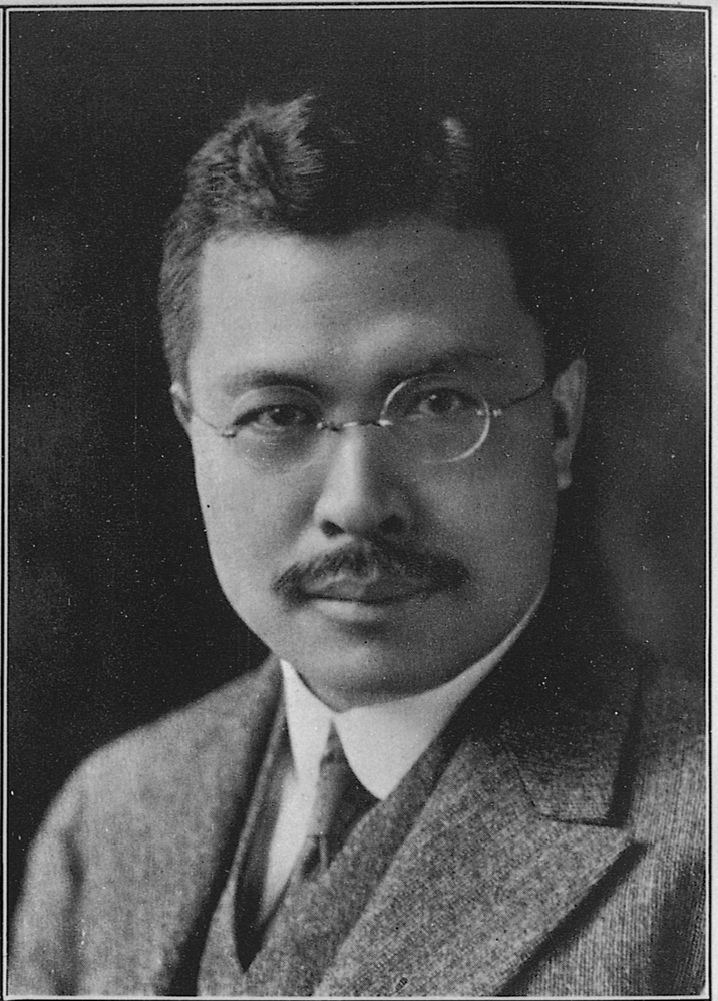
\includegraphics[scale=0.7]{Glava6/tX8KCIWX7IM.jpg}
	%	\label{fig:scipion} % Unique label used for referencing the figure in-text\end{document}
	%	%\addcontentsline{toc}{figure}{Figure \ref{fig:placeholder}} % Uncomment to add the figure to the table of contents%----------------------------------------------------------------------------------------
	\caption{Кидзюро Сидэхара в годы работы в Соединённых Штатах}%	CHAPTER 2
\end{figure}

Но прежде, чем мы пойдём дальше, нужно сказать несколько слов о позиции англичан и о том, почему они пошли на фактический, а потом и формальный разрыв союза, который так долго и успешно объединял две островные державы. Чтобы это понять, надо сперва в ретроспективе взглянуть на то, зачем же этот альянс понадобился Британской империи изначально. Для этого вернёмся в середину XIX столетия – золотой век Англии, Викторианскую эпоху. Величие британцев базировалось на трёх китах.

Первый – промышленная мощь. Мастерская мира была таковой всю первую половину века, но с 1850-х всё более ощутимыми становились возможности конкурентов. Британия могла многое – но только не ограничить искусственно развитие производительных сил в масштабах всей Европы и Северной Америки. Сперва США и Франция, а затем США и Германия весьма активно покушались на английское первенство, при этом имея ряд весомых преимуществ. У Штатов – громадный внутренний рынок, изобилие ресурсов и сырья, равномерный рост потребления по мере заселения Дикого Запада. У Германии – активная и толковая роль государства в экономике, очень квалифицированная и образованная, но более дешевая, чем в Англии, рабочая сила, тесная связка промышленности с наукой. Британия активно и деятельно боролась, но постепенно её доля в мировом производстве неуклонно сокращалась, и в Лондоне понимали, что глобально с этим ничего поделать нельзя – только сократить темпы и цифры.

Второй кит – финансовое могущество. Фунт стерлинга был самой твёрдой валютой мира, Лондонский Сити – крупнейшим финансовым центром. Здесь позиции империи оставались непоколебимыми до самой мировой войны, но в первую очередь, благо ещё не существовало огромного самовоспроизводящегося сектора виртуальных денег, это было возможным благодаря тому, что Англия была и оставалась центром мирового товарообмена.

В свою очередь это было так виду наличия третьего кита – крупнейшего на свете флота, как военного, так и торгового. Британия не зря носила звание Владычицы морей. Она имела безоговорочно мощнейшие ВМС в наиболее “освоенном” океане – Атлантическом, тратя на это огромные средства, но успешно окупая расходы. Флот Канала и Средиземноморская эскадра были готовы блокировать по необходимости любой европейский порт. США до конца 1880-х не имели сильного флота. Индийский океан вовсе был практически внутренним для англичан – ни одна другая великая морская держава не имела там серьёзных баз и сил. Только французы завладели в итоге Мадагаскаром и Джибути, но это, во-первых случилось только под самый конец века, во-вторых, так и не привело к созданию сколь либо серьёзной военно-морской инфраструктуры в регионе. Но оставался ещё Тихий океан (Северный ледовитый по понятным причинам можно не рассматривать). У Британии и там были весьма удачно расположенные и хорошо оборудованные пункты базирования: Сингапур, Гонконг, в меньшей степени Сидней. Но вот флотов на плотный контроль самого большого и, как назло, самого отдалённого от берегов Альбиона океана уже не хватало. До постройки Суэцкого канала силы в регионе и вовсе были мизерными.

Меж тем к середине 1850-х удобный выход в Тихий океан получили две основных страны-противника Британии. В 1848 году в ходе американо-мексиканской войны его приобрёл основной экономический соперник – США. В 1858 и 1860 годах по Айгуньскому и Пекинскому договорам получает Приморье главный военный противник – Российская империя. Наиболее дальновидные умы в Англии понимают – да, сейчас и у русских, и у американцев сильного флота в Тихом океане нет. Но он неизбежно появится рано или поздно. Через 15-20, пусть 25 лет, но он будет. А для Англии это по-прежнему будет обратная сторона Земли, периферия. И даже если империя и сможет выслать туда значительные силы без угрозы оголения и ослабления своих позиций в других двух океанах, всё равно этих сил окажется недостаточно для противостояния двум таким могущественным противникам сразу. Требовалось иное решение. Требовался союзник, равно враждебный и русским и американским притязаниям, которые могут возникнуть в регионе. Но вот беда – нет такого союзника. Франция, завладевшая Индокитаем (Вьетнам, Лаос) – конкурент Британии и не станет ей помогать за просто так, да и в принципе у неё нет никаких оснований ввязываться в конфликт с США или Россией. Испания чувствует угрозу со стороны Штатов своим колониальным владениям, но не станет искать ссоры с русскими. Ни одно из государств Южной Америки не подходит – они тоже не захотят, не смогут и не станут сдерживать Россию. Китай враждебен Англии и очень ею ослаблен. И вообще сознательно усиливать Поднебесную… это может плохо закончиться. Остальные государства, имеющие выход в Тихий океан, слишком дикие и слабые. Или нет? Япония в 1860-е вступает на путь обновления и реформ, она достаточно густо населена и очень выгодно географически расположена. Она охватывает российские владения, имеющие выход к морю, при этом, находясь на островах, защищена от атаки сухопутных сил, конечно, при наличии достаточно сильного флота. С США сложнее – японцы всё же далековато, чтобы служить полноценным сдерживающим фактором. С другой стороны, Штаты тоже не смогут им особенно угрожать, при этом вовсе не учитывать Японию у них не получится.

И Британия начинает реализацию грандиозного политического плана: она сознательно растит себе союзника. Это вообще было совершенно нетипично для британской дипломатической традиции – не временный ситуативный альянс, в основе которого ловкость посланников, деньги и некая общая угроза, не клиент-сателлит, готовый покорно исполнять волю патрона, но почти равноправный партнёр со своими интересами, которые чем дальше, тем больше нужно будет учитывать. Формальный союз возникнет только в 1902, но фактически англичане начнут опекать Японию гораздо раньше. Они строят и в организационном, и в фактическом смысле флот Страны Восходящего солнца, они помогают ускоренному преобразованию производства и общественной жизни. Влияние их очень велико – и даже японские школьницы получат костюмчики, в основе которых лежит униформа британских матросов 1880-х.

Дерзкий проект себя полностью оправдывает. Япония становится действенным фактором против российской экспансии, а в конечном счёте в ходе Русско-японской войны её практически останавливает. С США дела обстояли сложнее. Испано-американская война показала резкий рост и военно-морской силы Штатов и их притязаний. У англичан не было ни особенного желания вытягивать совершенно деградировавшую в военном отношении Испанию, ни реальной возможности это сделать. Ну а с начала XX века внимание Лондона всё больше поглощает противоборство с Берлином. В итоге выходит, что военно-морское давление на США с двух океанов, с двух огромных фронтов – Королевским флотом из Атлантики и японскими силами с Тихого океана, так никогда и не реализуется, даже в виде угрозы, возможности. Свою роль сыграла и слишком маленькая дистанция между Русско-японской и Первой мировой. Сперва японцы никак не могли затевать конфликт, чреватый тяжёлой войной с новым противником, а потом полностью заняты борьбой с Центральными державами оказались уже британцы. Вообще США в Первую мировую идеально реализовала стратегию сидящей на горе мудрой обезьяны, глядящей, как внизу дерутся тигры. К концу ПМВ и особенно после краха Восточного фронта Антанта оказалась полностью зависима от воли Вашингтона.

Можно было бы думать, что уже после победы ситуация изменится, но… Были иные, невоенные факторы. Первый - долги - английское правительство имело долг перед США в размере 4,5 миллиардов долларов. И исключительно от доброй воли Вашингтона зависело как именно и в какой срок Лондон будет расплачиваться. Во вторых за время Первой мировой именно США сделались впервые за добрых два века потеснив Англию, лидером по торговому морскому тоннажу и объёму перевозок. Резко прибавил и военный флот, хотя и уступающий пока Гранд Флиту, но, после гибели немецкого флота Открытого моря, второй по силе в мире. И главное – американские темпы постройки и спуска были примерно равны английским и даже несколько превосходили их. В период с августа 1914 и до начала Вашингтонской конференции в США было введено в строй 13 новых дредноутов, а в Британии – 12. Причём в 1921 Штаты заложили рекордную серию из сразу 6 новых линкоров, готовность которых к моменту окончания конференции составит примерно 30\%, а сроком достройки всей серии должен был стать 1923 год. 

\begin{figure}[h!tb] 
	\centering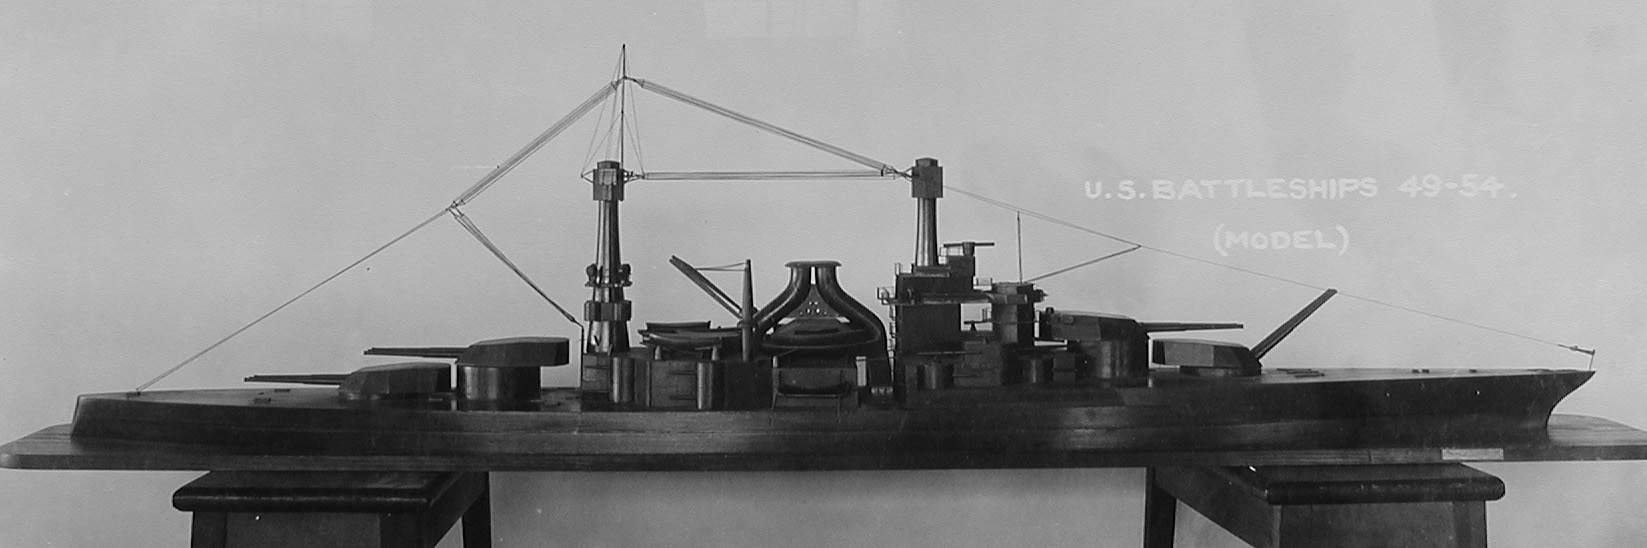
\includegraphics[scale=0.2]{Glava6/tdsTMXV67x0.jpg}
	%	\label{fig:scipion} % Unique label used for referencing the figure in-text\end{document}
	%	%\addcontentsline{toc}{figure}{Figure \ref{fig:placeholder}} % Uncomment to add the figure to the table of contents%----------------------------------------------------------------------------------------
	\caption{Макет одного из недостроенных линкоров}%	CHAPTER 2
\end{figure}

В свою очередь Британия пока ещё только обсуждала и готовила проекты новых, пусть и очень мощных, линейных крейсеров и дредноутов. При этом, если возможности верфей и в целом военно-морской промышленности США и Альбиона были сопоставимы, то удельный вес расходов и в целом финансовая состоятельность стран очень сильно отличалась. Британия желала передышки, люди слышать больше не хотели о новых военных расходах, а здесь налицо был риск начать новую дредноутную гонку, да как бы не более напряжённую и тяжёлую, чем гонка с Германией. Причём все помнили, конечно, что это состязание в числе прочих факторов сыграло видную роль в прокладывании дороги к войне. Огромная часть элит, надеющихся на приток американских капиталов, скорее дала бы себя прилюдно выпороть, чем испортить отношения с Америкой. В массах крепло влияние лейбористов, важным программным пунктом которых была антивоенная тема.

Впрочем, кроме долгов и риска новой дредноутной гонки было и ещё кое-что. Война сильно увеличила степень экономической независимости колоний от метрополии, показала, до какой степени вторая нуждается в первых. Никогда прежде Британия так активно не пользовалась войсками, происходившими не из Альбиона. Новозеландцы и австралийцы сражались на пляжах Галипполи, канадцы тонули в грязи Фландрии, и теперь чувствовали себя вправе на свою – и именно свою, долю в плодах победы. Созданные для того, что в зародыше подавить угрозу сепаратизма в рамках империи (и справлявшиеся с этой задачей в мирное время) после войны правительства Доминионов стали сами всё сильнее проявлять его. Некогда формально имевшиеся полномочия стали наполняться реальным содержанием. Вообще, объективно говоря, очень сложно сказать, что было бы большим злом для Британии – то, что произошло в реальности, или неучастие страны в Первой Мировой вообще. Опасаясь конкуренции с германской промышленностью, к 1921 англичане вчистую проиграли её промышленности штатовской. Экономические связи не только граничащей с США Канады, но и весьма удалённой Австралии со страной под звёздно-полосатым флагом стали примерно равны связям со страной под Юнион Джеком. Мало того, если немцы всё же вызывали бы неприятие чуждой культурой, иным языком, то в американцах тем же жителям Канады сложно было не признать пусть и давненько пошедшей своим путём, но родни.

Наконец, совершенно другим было отношение имевших выход к Тихому океану доминионов к японской экспансии. И Канада, и Австралия были крайне малонаселёнными, а потому мысль о том, что у испытывающей жесткую потребность в жизненном пространстве Японии появится флот, более сильный, чем всё, что англичане, или даже американцы смогут держать в тихоокеанских портах, приводила их в трепет.

Одним словом, масса факторов толкала англичан к некоему компромиссу с американцами, благо они сами его предлагали. Соглашение по морским вооружениям и уничтожение англо-японского союза гарантировало мир, возможность изрядно сэкономить на вооружениях, а главное закрепляла соотношение флотов США и Британии как 1 к 1. Попытки же бороться за прежний статус и безусловное, единоличное первенство могли привести к потере и того, что уже было. Ну а полновесная война и вовсе была чревата массой рисков – от внутреннего восстания истощенного войнами населения и до резкого толчка вперёд пока ещё только намеченной США темы права народов на самоопределение и деколонизации.

И всё же выбор для Англии был крайне неоднозначным. 1921 год – одна из важных развилок мировой истории. Согласившись на условия Вашингтона, англичане по сути гарантировали своему имперскому величию тихую старость и почётную смерть. Если США вполне были готовы к экспансии чисто экономическими методами, силами доллара и Форда, то для Британии единственной возможностью сохранить свои позиции была опора на силу – чисто военную, обилие ресурсов, широту охвата станций и баз. Кроме того, империя была бы не одна – те же японцы до последнего надеялись в ходе конференции на старый союз и сохраняли ему верность. А после — не простили измены. Я убеждён – и это один из выводов данной серии, что если бы не Вашингтонская конференция, не разрыв англо-японского союза, не унижение, которое испытали японцы, они никогда не оказались бы в следующей мировой войне в числе врагов Британии и в одной лодке с Германией и Италией. А возможно Вторая Мировая вообще не началась бы, потому что корни политики умиротворения для англичан именно здесь в готовности сдать союзника (как потом сдадут Чехословакию) и стратегические цели во имя пусть немалой, но всё же тактической выгоды.

Подробности хода Вашингтонской конференции, отголоски её решений в японской внутренней политике и судьба флотских программ Страны Восходящего солнца в условиях принятых ограничений – в следующей части.

\url{https://vk.com/wall-162479647_83571}